\documentclass[a4paper,11pt]{article}
\usepackage{lmodern}			% Usa a fonte Latin Modern
\usepackage[T1]{fontenc}		% Seleção de códigos de fonte
\usepackage[utf8]{inputenc}		% Codificação do documento
\usepackage[brazil]{babel}
\usepackage{indentfirst}		% Indenta o primeiro parágrafo de cada seção.
\usepackage{graphicx}			% Inclusão de gráficos
\usepackage{subfig}				% enables the use of subfigures in floats
\usepackage{float}
\usepackage[
%	a4paper,
left=2cm,
right=1.5cm,
bottom=1.5cm,
top = 2.5cm,
foot=0.7cm]{geometry}
\usepackage{url}
\usepackage{setspace}
\usepackage{amsmath}
\usepackage{amsfonts}
\usepackage{fancyhdr}
\usepackage{multirow}
\usepackage{tabularx}
\usepackage{natbib}
\usepackage{enumitem}
\usepackage{graphicx}
\usepackage{subcaption}

\bibliographystyle{abbrvnat}
\setcitestyle{open={(},close={)}}
 %Citation-related commands

\usepackage{hyperref}

\usepackage{listings}
\usepackage{xcolor}
\usepackage[titletoc]{appendix}
\usepackage{array}
% Coluna numerica de largura fixa e centralizada (espacamento uniforme entre colunas)
\newcolumntype{C}{>{\centering\arraybackslash}p{0.7cm}}



\lstset{
  language=Python,
  basicstyle=\ttfamily\small,
  keywordstyle=\color{blue},
  commentstyle=\color{gray},
  stringstyle=\color{red},
  numbers=left,
  numberstyle=\tiny\color{gray},
  stepnumber=1,
  numbersep=5pt,
  backgroundcolor=\color{backcolour},
  frame=single,
  breaklines=true,
  captionpos=b,
  tabsize=4
}

\definecolor{codegreen}{rgb}{0,0.6,0}
\definecolor{codegray}{rgb}{0.5,0.5,0.5}
\definecolor{codepurple}{rgb}{0.8,0,0.2}
\definecolor{backcolour}{rgb}{.95,.95,1}

\lstdefinestyle{mystyle}{
    backgroundcolor=\color{backcolour},
    commentstyle=\color{codegreen},
    keywordstyle=\color{blue},
    numberstyle=\tiny\color{codegray},
    stringstyle=\color{codepurple},
    basicstyle=\ttfamily\footnotesize,
    breakatwhitespace=false,
    breaklines=true,
    captionpos=b,
    keepspaces=true,
    numbers=left,
    numbersep=5pt,
    showspaces=false,
    showstringspaces=false,
    showtabs=false,
    tabsize=2,
    language=Python
}

\pagestyle{fancy}
\fancyhf{}
\lhead{\small INE410159 -- Visão Computacional}
\rhead{\small Relatório - Detecção de anomalias em painéis solares}
\rfoot{\thepage}

\begin{document}
\onehalfspacing
\thispagestyle{empty}
\begin{center}
	
\includegraphics[height=2cm]{logoUFSCsimples} \\
	{\large Universidade Federal de Santa Catarina -- UFSC} \\
	{\large Centro Tecnológico -- CTC} \\
	{\large Departamento de Informática e Estatística -- INE} \\
	\vspace{1cm}
	INE410159 -- Visão Computacional \\
	\vfill
	\textbf{DETECÇÃO DE ANOMALIAS EM PAINÉIS SOLARES \\ UTILIZANDO TÉCNICAS DE VISÃO COMPUTACIONAL} \\
	\vspace{1cm}
	Autores: \\
	Gabriel Vinicius Crippa - 20206969 \\
	Gustavo Portela Alves - 21100467 \\
	Júlia Sebold May - 21101148 \\
	Yuri Melo Nunes - 20104163 \\
	\vfill
	Florianópolis, \today.
\end{center}

\clearpage

\tableofcontents

\clearpage

\section{Introdução}
A transição energética tem impulsionado a adoção de fontes de energia limpa e renovável. Os sistemas fotovoltaicos se destacam como uma das principais alternativas dentro da expansão das fontes renováveis, sendo amplamente empregados em instalações residenciais e comerciais. Esses sistemas utilizam módulos solares para converter diretamente a radiação solar em energia elétrica, permitindo a geração distribuída e reduzindo a dependência de fontes convencionais de energia.

Durante sua vida útil, os módulos fotovoltaicos estão sujeitos a intempéries e desgastes operacionais que podem gerar anomalias, comprometendo o potencial de geração de energia. Atualmente, a identificação e a correção dessas falhas dependem de inspeções termográficas periódicas. A abordagem convencional envolve a medição manual em campo utilizando câmeras termográficas portáteis, enquanto soluções mais modernas empregam drones equipados com sensores térmicos. Embora a utilização de drones agilize a captura de dados, o processo ainda exige que as imagens sejam analisadas individualmente pelo olhar humano de um técnico, que inspeciona visualmente os registros para diagnosticar as anomalias e direcionar as estratégias de manutenção.

O diagnóstico visual realizado por operadores humanos pode se tornar um processo demorado e suscetível a falhas ou inconsistências. Como sugestão de aprimoramento, este trabalho propõe a aplicação de técnicas de visão computacional para a análise de imagens termográficas de painéis solares. Por meio da integração de abordagens de visão clássica e algoritmos de aprendizado profundo, o objetivo é facilitar e acelerar a detecção de anomalias, fornecendo uma ferramenta mais robusta e eficiente para o diagnóstico de falhas nesses sistemas.
\clearpage

\section{Dataset}
Para o desenvolvimento e treinamento dos modelos de visão computacional, este trabalho utiliza o conjunto de dados público denominado \textit{InfraredSolarModules}. Este \textit{dataset} foi escolhido por fornecer imagens reais em infravermelho de diversas anomalias encontradas em usinas de geração solar. A literatura carece de bases de dados termográficas em larga escala disponíveis publicamente; portanto, a utilização desse \textit{dataset} supre essa lacuna, viabilizando pesquisas em aprendizado de máquina voltadas para a otimização e eficiência da indústria fotovoltaica.

O \textit{dataset} é composto por 20.000 imagens termográficas, cada uma possuindo uma resolução espacial de 24 por 40 pixels. Os dados estão estruturados e categorizados em 12 classes distintas que descrevem o estado de operação dos painéis. Dentre elas, 11 classes representam diferentes tipos de falhas ou degradações detectáveis por assinaturas térmicas, enquanto a classe restante, denominada "Sem Anomalia" (\textit{No-Anomaly}), representa o caso nulo de um módulo operando em condições nominais. Os rótulos de cada amostra são organizados em um arquivo estruturado (JSON), que relaciona o diretório da imagem à sua respectiva classe de anomalia.

A Tabela \ref{tab:classes_dataset} detalha as classes presentes na base de dados, a quantidade de imagens disponíveis para cada categoria e a descrição do comportamento termográfico associado.

\begin{table}[htpb]
	\centering
	\caption{Distribuição e descrição das classes de anomalias no dataset \textit{InfraredSolarModules}.}
	\label{tab:classes_dataset}
	\vspace{0.2cm}
	\begin{tabular}{l c p{9cm}}
		\hline
		\textbf{Classe} & \textbf{Imagens} & \textbf{Descrição}                                                                      \\
		\hline
		Cell            & 1.877            & Ponto quente com geometria quadrada ocorrendo em uma única célula.                      \\
		Cell-Multi      & 1.288            & Pontos quentes com geometria quadrada ocorrendo em múltiplas células.                   \\
		Cracking        & 941              & Anomalia no módulo causada por rachaduras em sua superfície.                            \\
		Hot-Spot        & 251              & Ponto quente isolado em um módulo de filme fino (\textit{thin film}).                   \\
		Hot-Spot-Multi  & 247              & Múltiplos pontos quentes em um módulo de filme fino.                                    \\
		Shadowing       & 1.056            & Obstrução da luz solar causada por vegetação, outras estruturas ou fileiras de painéis. \\
		Diode           & 1.499            & Diodo de desvio (bypass) ativado, afetando tipicamente 1/3 do módulo.                   \\
		Diode-Multi     & 175              & Múltiplos diodos de desvio ativados, afetando tipicamente 2/3 do módulo.                \\
		Vegetation      & 1.639            & Painéis obstruídos pelo crescimento de vegetação.                                       \\
		Soiling         & 205              & Presença de terra, poeira ou outros detritos acumulados na superfície do módulo.        \\
		Offline-Module  & 828              & Módulo inativo, caracterizado pelo aquecimento de toda a sua extensão.                  \\
		No-Anomaly      & 10.000           & Módulo solar operando em condições nominais, sem defeitos.                              \\
		\hline
	\end{tabular}
\end{table}
\clearpage

\section{Solução com visão clássica}

\subsection{Preparação do ambiente e análise exploratória dos dados}

O desenvolvimento do projeto foi centralizado na plataforma \textit{Google Colab}, utilizando uma abordagem modular dividida em seções sequenciais. O conjunto de dados \textit{InfraredSolarModules} foi importado diretamente do repositório remoto para o ambiente virtual de execução, sendo o arquivo \textit{module\textunderscore metadata.json} convertido em uma estrutura de tabela (\textit{DataFrame} do \textit{Pandas}) para correlacionar cada arquivo de imagem de 24x40 pixels à sua respectiva classe de anomalia.

Foi desenvolvida uma rotina para visualização e inspeção visual das matrizes brutas em tons de cinza. Durante esse processo de análise exploratória, identificou-se um comportamento indesejado de renderização da biblioteca \textit{Matplotlib} (\textit{pyplot.imshow}). Por padrão, a biblioteca aplica uma normalização automática de contraste baseada exclusivamente nos valores mínimos e máximos locais de cada imagem.

Essa característica fazia com que a visualização fosse prejudicada, painéis categorizados como nominais (\textit{No-Anomaly}) apresentavam manchas e gradientes de calor inexistentes no mundo real, uma vez que variações irrelevantes eram esticadas para preencher toda a escala visual. A resolução desse problema e a calibração correta dos dados exigiram o travamento explícito dos limites de exibição nos valores absolutos do sensor infravermelho, utilizando os parâmetros matemáticos $vmin=0$ e $vmax=255$. A Figura \ref{fig:comp_escala} ilustra o impacto dessa correção, revelando a assinatura térmica uniforme real de um módulo saudável.

\begin{figure}[H]
	\centering
	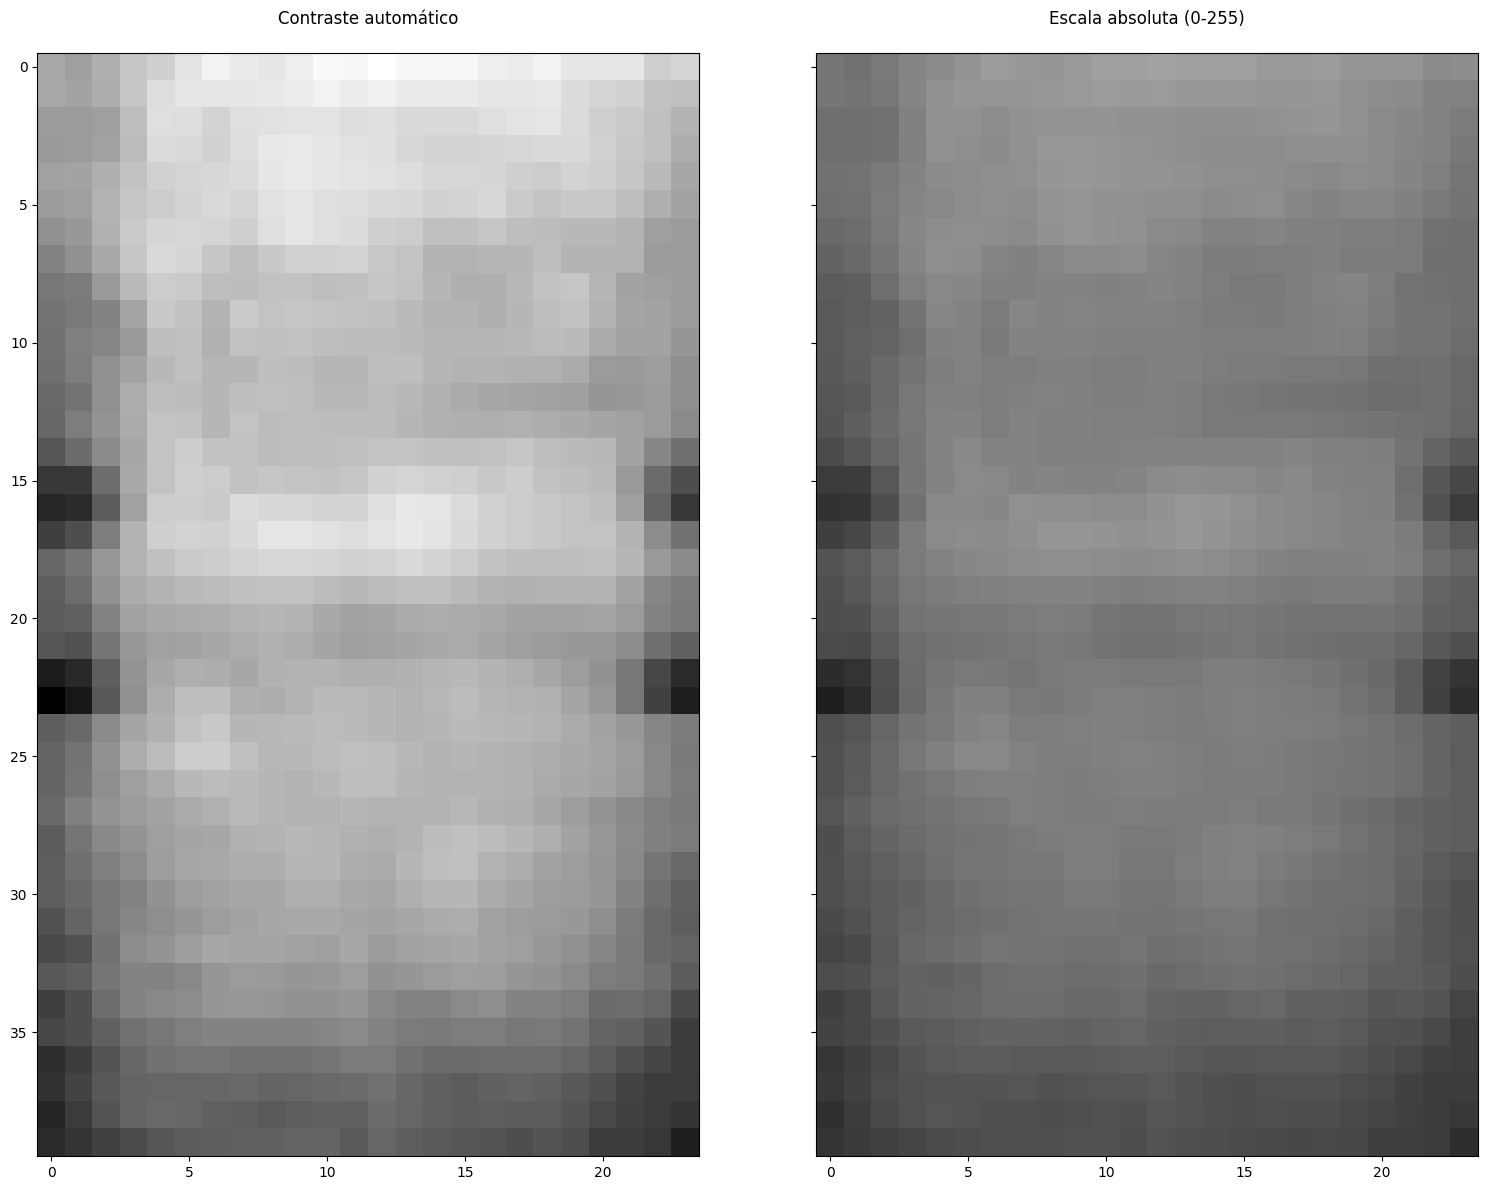
\includegraphics[width=0.5\linewidth]{comp_escala.png}
	\caption{Impacto da normalização automática versus escala térmica absoluta (0-255) em módulo nominal.}
	\label{fig:comp_escala}
\end{figure}

\subsection{\textit{Pipeline} de análise inicial}

A partir da estabilização visual dos dados, estabeleceu-se que os defeitos baseados em superaquecimento geométrico estrito (notadamente a classe \textit{Cell}) possuíam forte assinatura no domínio do valor. Foi desenhado e implementado um \textit{pipeline} clássico composto por quatro etapas sequenciais utilizando a biblioteca \textit{OpenCV}:

\begin{enumerate}
	\item \textbf{Limiarização binária} (\textit{cv2.threshold}): operando diretamente na intensidade dos pixels, aplicou-se um limiar de corte ($T = 180$). Pixels com intensidade superior a $T$ (zonas de alta temperatura) foram binarizados para branco (255), enquanto o restante da estrutura do painel foi mapeado para preto (0).
	\item \textbf{Condicionamento espacial por morfologia matemática} (\textit{cv2.morphologyEx}): na sequência utilizou-se uma operação morfológica composta de abertura (uma filtragem de erosão seguida por dilatação). Dado o tamanho reduzido das imagens (24x40 pixels), calibrou-se um elemento estruturante (\textit{kernel}) compacto de dimensões $2\times2$ preenchido por uns. A erosão eliminou os pixels isolados de ruído, enquanto a subsequente dilatação restaurou a massa geométrica da anomalia principal.
	\item \textbf{Extração de características e medição de contornos} (\textit{cv2.findContours}): a imagem binária condicionada foi submetida a um algoritmo de varredura geométrica para identificar contornos externos. A partir das fronteiras localizadas, calculou-se a área em pixels da maior mancha quente de cada imagem por meio da função \textit{cv2.contourArea}.
	\item \textbf{Classificação heurística baseada em regras:} como fechamento da lógica, estruturou-se um decisor heurístico simples fundamentado na dimensão da área segmentada:
	      \begin{itemize}
		      \item Se a maior área fosse inferior a 5 pixels, o módulo era classificado como \textit{No-Anomaly};
		      \item Se a área superasse 700 pixels (indicando que praticamente toda a matriz 24x40 atingiu saturação térmica), o módulo era mapeado como \textit{Offline-Module};
		      \item Áreas intermediárias sobreviventes eram rotuladas como anomalias puntiformes da classe \textit{Cell}.
	      \end{itemize}
\end{enumerate}

\subsection{Extração de características e comparação de classificadores}

Após o teste inicial focado na classe \textit{Cell}, optou-se por uma abordagem de aprendizado de máquina, na qual cada imagem é convertida em um vetor de características. Definiu-se um conjunto inicial de 25 características:

\begin{itemize}[noitemsep]
	\item \textbf{Estatísticas de intensidade}: média, desvio padrão, máximo, mínimo e percentil 90 dos pixels.
	\item \textbf{Fração de região quente}: proporção de pixels acima do limiar de Otsu.
	\item \textbf{Número de manchas}: quantidade de regiões quentes distintas.
	\item \textbf{Geometria da maior mancha}: área, extensão e razão de aspecto.
	\item \textbf{Cobertura por linha e coluna}: espalhamento vertical e horizontal do calor.
	\item \textbf{Fração de região fria}: proporção de pixels bem abaixo da média.
	\item \textbf{Densidade de bordas}: contornos detectados pelo operador \textit{Canny}.
	\item \textbf{Textura}: magnitude média do gradiente (operador de \textit{Sobel}).
	\item \textbf{Simetria}: diferença da imagem em relação a si espelhada na horizontal e na vertical.
	\item \textbf{Histograma}: distribuição de intensidades em oito faixas.
\end{itemize}

Sobre esse conjunto, avaliaram-se quatro classificadores:

\begin{itemize}[noitemsep]
	\item \textbf{Random Forest}: conjunto de árvores de decisão combinadas por agregação (\textit{bagging}).
	\item \textbf{Gradient Boosting}: árvores em sequência, cada uma corrigindo o erro da anterior.
	\item \textbf{SVM}: busca a fronteira de maior margem entre as classes; exige normalização das características.
	\item \textbf{XGBoost}: \textit{gradient boosting} otimizado, robusto em dados tabulares.
\end{itemize}

Todos foram treinados com tratamento do desbalanceamento e avaliados na mesma partição de teste (30\%, estratificada). Adota-se o \textit{F1-score} macro como métrica principal, por pesar todas as classes igualmente. A Tabela \ref{tab:f1_classe_base} detalha a \textit{precision} (P), o \textit{recall} (R) e o \textit{F1-score} (F1) por classe de cada modelo, permitindo localizar onde cada classificador acerta ou falha.

\begin{table}[H]
	\centering
	\caption{\textit{Precision} (P), \textit{recall} (R) e \textit{F1-score} (F1), em \%, por classe e por modelo sobre o conjunto base de características.}
	\label{tab:f1_classe_base}
	\vspace{0.2cm}
	\setlength{\tabcolsep}{6pt}
	\renewcommand{\arraystretch}{1.25}
	\resizebox{\textwidth}{!}{%
	\begin{tabular}{l|CCCC|CCCC|CCCC}
		\hline
		                & \multicolumn{4}{c|}{\textbf{Precision}} & \multicolumn{4}{c|}{\textbf{Recall}} & \multicolumn{4}{c}{\textbf{F1-score}} \\
		\textbf{Classe} & RF & GB & SVM & XGB & RF & GB & SVM & XGB & RF & GB & SVM & XGB \\
		\hline
		Cell            & 46 & 44 & 46 & 49 & 45 & 41 & 35 & 48 & 46 & 43 & 40 & 48 \\ \hline
		Cell-Multi      & 36 & 35 & 35 & 36 & 25 & 29 & 17 & 28 & 29 & 32 & 22 & 32 \\ \hline
		Cracking        & 59 & 57 & 59 & 63 & 73 & 69 & 68 & 69 & 65 & 62 & 63 & 66 \\ \hline
		Diode           & 54 & 53 & 58 & 69 & 70 & 65 & 57 & 66 & 61 & 58 & 58 & 67 \\ \hline
		Diode-Multi     & 39 & 19 &  7 & 39 & 21 & 29 & 35 & 13 & 28 & 23 & 11 & 20 \\ \hline
		Hot-Spot        & 26 &  8 &  4 & 23 & 13 & 23 & 41 &  7 & 18 & 11 &  8 & 10 \\ \hline
		Hot-Spot-Multi  & 28 & 20 &  8 & 47 & 38 & 43 & 42 & 34 & 32 & 28 & 14 & 39 \\ \hline
		No-Anomaly      & 82 & 84 & 85 & 78 & 76 & 62 & 41 & 89 & 79 & 71 & 56 & 83 \\ \hline
		Offline-Module  & 29 & 25 & 21 & 44 & 46 & 46 & 46 & 33 & 36 & 32 & 28 & 38 \\ \hline
		Shadowing       & 40 & 30 & 28 & 49 & 48 & 49 & 54 & 38 & 44 & 37 & 37 & 43 \\ \hline
		Soiling         & 26 & 19 & 13 & 22 & 16 & 25 & 36 & 10 & 20 & 21 & 19 & 14 \\ \hline
		Vegetation      & 46 & 41 & 41 & 47 & 46 & 45 & 39 & 43 & 46 & 43 & 40 & 45 \\
		\hline
	\end{tabular}%
	}
\end{table}

A Tabela \ref{tab:benchmark_base} resume o desempenho geral de cada modelo.

\begin{table}[H]
	\centering
	\caption{Comparação dos classificadores sobre o conjunto base de 25 características.}
	\label{tab:benchmark_base}
	\vspace{0.2cm}
	\begin{tabular}{l c c}
		\hline
		\textbf{Modelo} & \textbf{Acurácia} & \textbf{F1-score macro} \\
		\hline
		XGB             & 66,6\%            & 42,2\%                  \\
		RF              & 61,9\%            & 41,9\%                  \\
		GB              & 54,3\%            & 38,5\%                  \\
		SVM             & 42,0\%            & 32,9\%                  \\
		\hline
	\end{tabular}
\end{table}

Os resultados evidenciam a superioridade dos métodos baseados em árvores, com destaque para o \textit{XGBoost}, que obteve o melhor desempenho tanto em acurácia quanto em \textit{F1-score} macro. O salto em relação à heurística inicial confirma a vantagem de combinar múltiplas características com um classificador treinado. Ainda assim, os valores relativamente modestos do \textit{F1-score} macro indicam dificuldade na distinção entre classes minoritárias e visualmente semelhantes, o que motiva o refinamento do conjunto de características descrito na seção seguinte.

\subsection{Refinamento incremental das características}

Como o \textit{Random Forest} (RF) e o \textit{XGBoost} (XGB) mostraram-se muito superiores ao \textit{Gradient Boosting} e ao SVM no benchmark anterior, o restante da análise prossegue apenas com esses dois modelos. Investigou-se o impacto de enriquecer o vetor de características: partindo do conjunto base de 25 atributos, novos grupos foram incorporados \textbf{de forma cumulativa} (cada etapa mantém os grupos anteriores e adiciona um novo), medindo-se a acurácia e o \textit{F1-score} macro a cada adição. Assim, a última linha das tabelas (181 features) corresponde a \textbf{todas as características em conjunto}. Os grupos acrescentados, nesta ordem, foram:

\begin{itemize}[noitemsep]
	\item \textbf{Grade 3x3 + LBP}: intensidade média em uma grade de nove células (localização do calor) e \textit{Local Binary Patterns} (textura local).
	\item \textbf{Skewness e kurtosis}: assimetria e concentração da distribuição de intensidades.
	\item \textbf{Momentos de Hu}: descritores de forma da maior mancha, invariantes a escala e rotação.
	\item \textbf{Gabor + HOG}: resposta a filtros de Gabor (textura direcional) e histograma de gradientes orientados (formas e trincas).
\end{itemize}

A coluna $\Delta$ indica a variação em relação ao conjunto base. As Tabelas \ref{tab:incremental_rf} e \ref{tab:incremental_xgb} apresentam a evolução para o RF e o XGBoost, respectivamente.

\begin{table}[H]
	\centering
	\caption{Refinamento incremental das características --- \textbf{Random Forest}.}
	\label{tab:incremental_rf}
	\vspace{0.2cm}
	\renewcommand{\arraystretch}{1.2}
	\begin{tabular}{l c c c c c}
		\hline
		\textbf{Conjunto de características} & \textbf{Nº feat.} & \textbf{Acurácia} & \textbf{$\Delta$} & \textbf{F1 macro} & \textbf{$\Delta$} \\
		\hline
		Base                 & 25  & 61,9\% & --     & 41,9\% & --     \\ \hline
		+ Grade 3x3 + LBP    & 44  & 65,1\% & +3,2   & 43,3\% & +1,3   \\ \hline
		+ Skewness/Kurtosis  & 46  & 64,9\% & +3,0   & 43,5\% & +1,6   \\ \hline
		+ Momentos de Hu     & 53  & 65,3\% & +3,4   & 44,3\% & +2,3   \\ \hline
		+ Gabor + HOG        & 181 & 67,8\% & +5,9   & 48,9\% & +7,0   \\
		\hline
	\end{tabular}
\end{table}

\begin{table}[H]
	\centering
	\caption{Refinamento incremental das características --- \textbf{XGBoost}.}
	\label{tab:incremental_xgb}
	\vspace{0.2cm}
	\renewcommand{\arraystretch}{1.2}
	\begin{tabular}{l c c c c c}
		\hline
		\textbf{Conjunto de características} & \textbf{Nº feat.} & \textbf{Acurácia} & \textbf{$\Delta$} & \textbf{F1 macro} & \textbf{$\Delta$} \\
		\hline
		Base                 & 25  & 66,6\% & --     & 42,2\% & --     \\ \hline
		+ Grade 3x3 + LBP    & 44  & 69,7\% & +3,1   & 45,5\% & +3,4   \\ \hline
		+ Skewness/Kurtosis  & 46  & 70,4\% & +3,8   & 46,6\% & +4,4   \\ \hline
		+ Momentos de Hu     & 53  & 70,6\% & +4,0   & 47,6\% & +5,5   \\ \hline
		+ Gabor + HOG        & 181 & 74,2\% & +7,6   & 53,9\% & +11,7  \\
		\hline
	\end{tabular}
\end{table}

Em ambos os modelos o desempenho cresce de forma consistente a cada grupo, e o salto mais expressivo vem do par \textit{Gabor} + HOG, indicando que descritores de textura direcional e de forma capturam padrões que as estatísticas de intensidade isoladas não representam. O ganho é mais acentuado no XGBoost, cujo \textit{F1-score} macro sobe de 42,2\% para 53,9\% (+11,7 pontos), contra +7,0 pontos do Random Forest, confirmando o XGBoost como o melhor classificador para o conjunto completo de características.

\subsection{Classificação em duas etapas (Anomalia vs No-Anomaly)}

Dado o forte desbalanceamento da base, em que a classe \textit{No-Anomaly} representa metade das amostras, avaliou-se uma estratégia de classificação em \textbf{duas etapas}. Na primeira, um classificador binário decide apenas se há ou não anomalia (\textit{Anomalia} vs \textit{No-Anomaly}); na segunda, um segundo classificador, treinado somente com imagens de anomalia, determina o tipo específico. A motivação é retirar o peso da classe majoritária da decisão fina entre os tipos de defeito.

A Tabela \ref{tab:duas_etapas} compara o modelo único (que decide as 12 classes de uma vez) com a abordagem em duas etapas, para o RF e o XGBoost, usando o conjunto completo de 181 características.

\begin{table}[H]
	\centering
	\caption{Modelo único vs classificação em duas etapas.}
	\label{tab:duas_etapas}
	\vspace{0.2cm}
	\renewcommand{\arraystretch}{1.2}
	\begin{tabular}{l l c c}
		\hline
		\textbf{Modelo} & \textbf{Abordagem} & \textbf{Acurácia} & \textbf{F1-score macro} \\
		\hline
		RF  & Único       & 67,6\% & 47,7\% \\ \hline
		RF  & Duas etapas & 69,2\% & 47,5\% \\ \hline
		GB  & Único       & 66,8\% & 48,3\% \\ \hline
		GB  & Duas etapas & 71,0\% & 48,5\% \\ \hline
		SVM & Único       & 64,7\% & 50,4\% \\ \hline
		SVM & Duas etapas & 71,6\% & 51,6\% \\ \hline
		XGB & Único       & 74,2\% & 53,9\% \\ \hline
		XGB & Duas etapas & 73,3\% & 52,9\% \\
		\hline
	\end{tabular}
\end{table}

Conclui-se que a divisão em duas etapas é mais valiosa como \textbf{detector de falhas} do que como melhoria da classificação fina, que permanece melhor servida pelo XGBoost único. A primeira etapa, isoladamente, constitui um detector de alto valor prático: responde se um painel precisa ou não de inspeção. A Tabela \ref{tab:detector} resume seu desempenho.

\begin{table}[H]
	\centering
	\caption{Desempenho do detector binário (etapa 1): anomalia vs \textit{No-Anomaly}.}
	\label{tab:detector}
	\vspace{0.2cm}
	\renewcommand{\arraystretch}{1.2}
	\begin{tabular}{l c c}
		\hline
		\textbf{Modelo} & \textbf{Acurácia} & \textbf{Recall de Anomalia} \\
		\hline
		RF  & 84,9\% & 79,6\% \\ \hline
		GB  & 86,5\% & 81,9\% \\ \hline
		SVM & 87,7\% & 83,2\% \\ \hline
		XGB & 88,4\% & 84,2\% \\
		\hline
	\end{tabular}
\end{table}

Apenas detectar a presença de uma possível falha, com 88,4\% de acurácia e recuperando 84,2\% das anomalias reais, já constitui um resultado de grande utilidade prática. Em uma usina solar, esse detector pode operar como um filtro automático que dispara um alerta sempre que um módulo apresenta indício de anomalia, encaminhando apenas os casos suspeitos para a verificação de um profissional. Assim, em vez de inspecionar manualmente todos os painéis, o técnico concentra o esforço nos módulos sinalizados pelo sistema, reduzindo drasticamente o volume de análise humana e agilizando a manutenção. Mesmo sem identificar o tipo exato do defeito, o simples acionamento confiável desse alerta representa um ganho operacional relevante para o monitoramento em larga escala.

\subsubsection{Ajuste do limiar de decisão}

Um aspecto importante desse detector é que o limiar de decisão pode ser ajustado conforme o objetivo da operação. Por padrão, um classificador atribui a classe \textit{Anomalia} quando a probabilidade estimada ultrapassa 0,5. Reduzir esse limiar torna o detector mais sensível: ele passa a sinalizar mais painéis como suspeitos, aumentando o \textit{recall} (proporção de falhas reais capturadas) ao custo de mais alarmes falsos (menor \textit{precision}). Para uma tarefa de triagem, esse compromisso é vantajoso, pois deixar de detectar uma falha real (falso negativo) costuma ser mais grave do que inspecionar um painel saudável (falso positivo). A Tabela \ref{tab:limiar} mostra esse trade-off para o detector XGBoost, variando o limiar de decisão.

\begin{table}[H]
	\centering
	\caption{\textit{Recall} e \textit{precision} da classe \textit{Anomalia} em função do limiar de decisão (detector XGBoost).}
	\label{tab:limiar}
	\vspace{0.2cm}
	\renewcommand{\arraystretch}{1.2}
	\begin{tabular}{c c c}
		\hline
		\textbf{Limiar} & \textbf{Recall} & \textbf{Precision} \\
		\hline
		0,50 & 84,2\% & 91,9\% \\ \hline
		0,40 & 85,8\% & 90,1\% \\ \hline
		0,30 & 87,8\% & 88,3\% \\ \hline
		0,20 & 90,2\% & 85,9\% \\ \hline
		0,10 & 92,8\% & 81,6\% \\
		\hline
	\end{tabular}
\end{table}

Reduzindo o limiar de 0,50 para valores menores, o \textit{recall} sobe progressivamente, permitindo capturar quase todas as anomalias ao custo de uma precisão menor. Na prática, isso significa que o operador pode calibrar o sistema para priorizar a segurança (não deixar passar falhas), aceitando inspecionar alguns painéis sãos a mais --- um ajuste desejável em um cenário de triagem automática.

\subsection{Análise das confusões entre classes (XGBoost)}

Confirmado o \textit{XGBoost} como o melhor classificador (74,2\% de acurácia e 53,9\% de \textit{F1-score} macro no conjunto completo), analisou-se em detalhe \textit{onde} o modelo erra. As Figuras \ref{fig:matriz_precision} e \ref{fig:matriz_recall} apresentam a matriz de confusão normalizada por coluna (\textit{precision}) e por linha (\textit{recall}), respectivamente. A primeira responde "do que foi previsto como classe X, quanto era X de fato"; a segunda, "da classe real X, quanto foi corretamente identificado".

\begin{figure}[H]
	\centering
	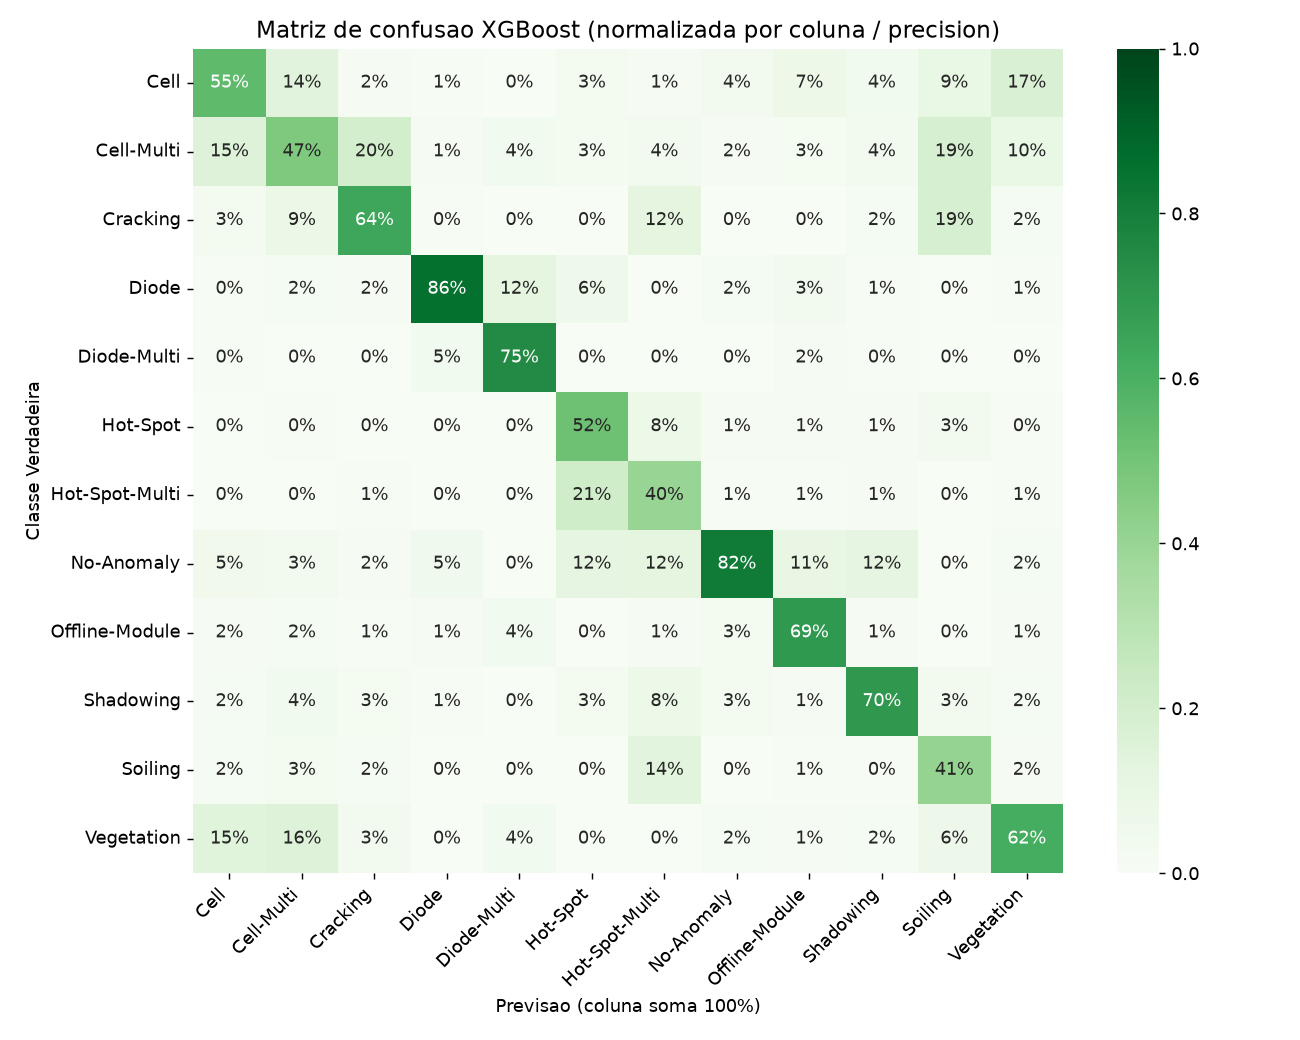
\includegraphics[width=0.8\linewidth]{matriz_xgb_precision.png}
	\caption{Matriz de confusão do XGBoost normalizada por coluna (\textit{precision}).}
	\label{fig:matriz_precision}
\end{figure}

\begin{figure}[H]
	\centering
	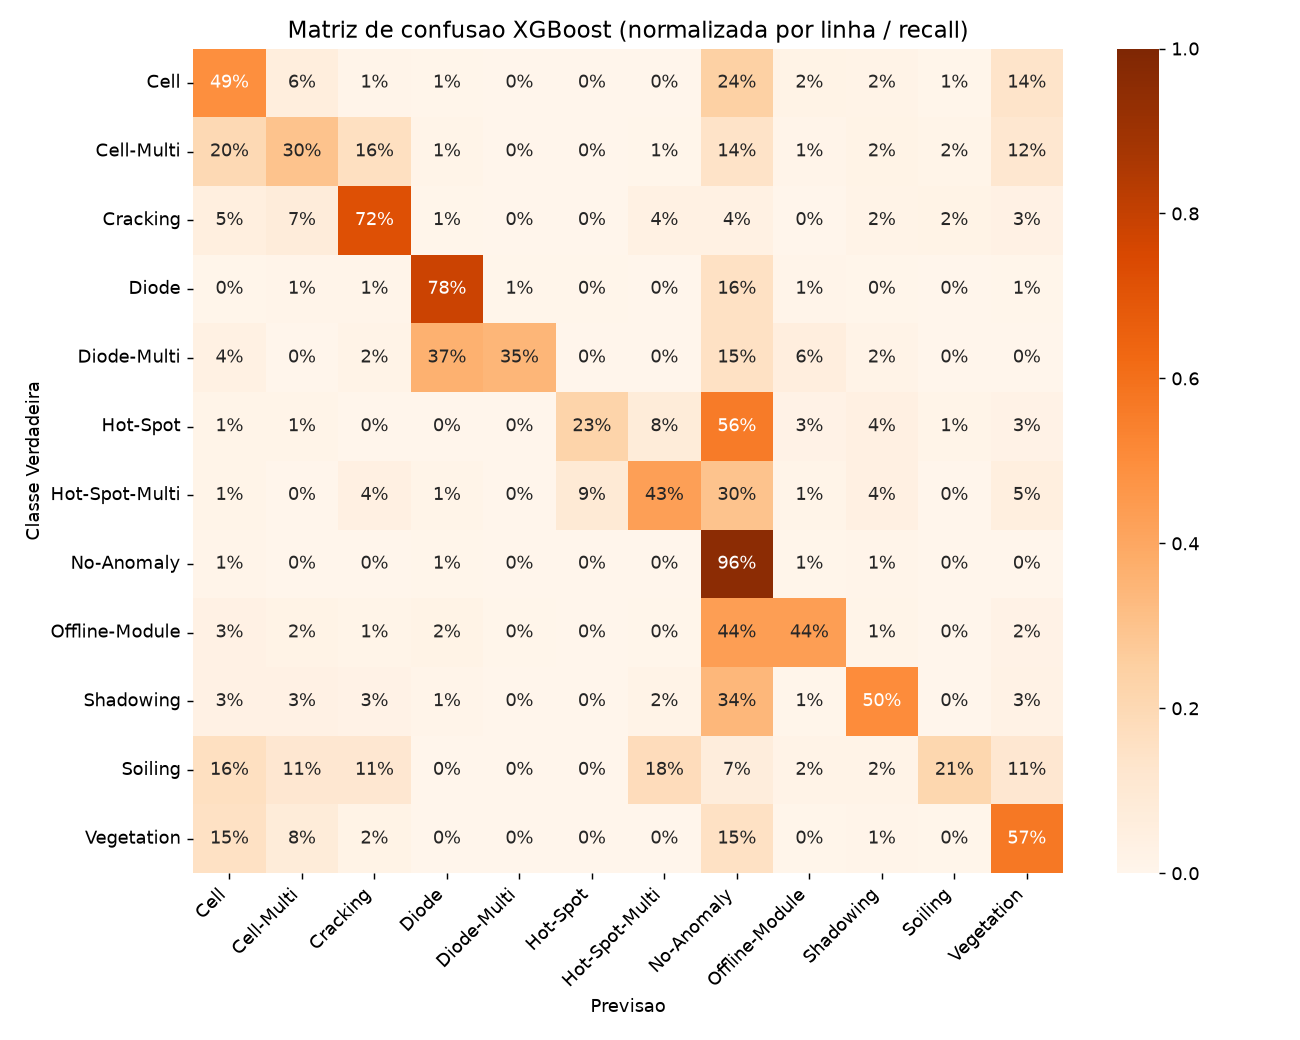
\includegraphics[width=0.8\linewidth]{matriz_xgb_recall.png}
	\caption{Matriz de confusão do XGBoost normalizada por linha (\textit{recall}).}
	\label{fig:matriz_recall}
\end{figure}

A partir da matriz por linha, a Tabela \ref{tab:confusoes} resume, para cada classe, o seu acerto próprio (\textit{recall}) e as cinco classes com as quais mais se confunde.

\begin{table}[H]
	\centering
	\caption{Cinco maiores confusões por classe (a partir da matriz de \textit{recall} do XGBoost).}
	\label{tab:confusoes}
	\vspace{0.2cm}
	\footnotesize
	\setlength{\tabcolsep}{4pt}
	\renewcommand{\arraystretch}{1.3}
	\resizebox{\textwidth}{!}{%
	\begin{tabular}{l r|l r|l r|l r|l r|l r}
		\hline
		\textbf{Classe} & \textbf{Acerto} & \multicolumn{2}{c|}{\textbf{1ª}} & \multicolumn{2}{c|}{\textbf{2ª}} & \multicolumn{2}{c|}{\textbf{3ª}} & \multicolumn{2}{c|}{\textbf{4ª}} & \multicolumn{2}{c}{\textbf{5ª}} \\
		\hline
		Cell           & 49\% & No-Anomaly & 24\% & Vegetation & 14\% & Cell-Multi & 6\% & Offline-Module & 2\% & Shadowing & 2\% \\ \hline
		Cell-Multi     & 30\% & Cell & 20\% & Cracking & 16\% & No-Anomaly & 14\% & Vegetation & 12\% & Shadowing & 2\% \\ \hline
		Cracking       & 72\% & Cell-Multi & 7\% & Cell & 5\% & No-Anomaly & 4\% & Hot-Spot-Multi & 4\% & Vegetation & 3\% \\ \hline
		Diode          & 78\% & No-Anomaly & 16\% & Offline-Module & 1\% & Cracking & 1\% & Cell-Multi & 1\% & Vegetation & 1\% \\ \hline
		Diode-Multi    & 35\% & Diode & 37\% & No-Anomaly & 15\% & Offline-Module & 6\% & Cell & 4\% & Shadowing & 2\% \\ \hline
		Hot-Spot       & 23\% & No-Anomaly & 56\% & Hot-Spot-Multi & 8\% & Shadowing & 4\% & Vegetation & 3\% & Offline-Module & 3\% \\ \hline
		Hot-Spot-Multi & 43\% & No-Anomaly & 30\% & Hot-Spot & 9\% & Vegetation & 5\% & Shadowing & 4\% & Cracking & 4\% \\ \hline
		No-Anomaly     & 96\% & Shadowing & 1\% & Cell & 1\% & Diode & 1\% & Offline-Module & 1\% & Hot-Spot-Multi & 0\% \\ \hline
		Offline-Module & 44\% & No-Anomaly & 44\% & Cell & 3\% & Vegetation & 2\% & Diode & 2\% & Cell-Multi & 2\% \\ \hline
		Shadowing      & 50\% & No-Anomaly & 34\% & Cell & 3\% & Cell-Multi & 3\% & Vegetation & 3\% & Cracking & 3\% \\ \hline
		Soiling        & 21\% & Hot-Spot-Multi & 18\% & Cell & 16\% & Vegetation & 11\% & Cracking & 11\% & Cell-Multi & 11\% \\ \hline
		Vegetation     & 57\% & Cell & 15\% & No-Anomaly & 15\% & Cell-Multi & 8\% & Cracking & 2\% & Shadowing & 1\% \\
		\hline
	\end{tabular}%
	}
\end{table}

Esta tabela é importante para futuras otimizações: indica possíveis agrupamentos e tratamentos específicos entre as classes. Os agrupamentos óbvios são \textit{Cell} com \textit{Cell-Multi}, \textit{Diode} com \textit{Diode-Multi} e \textit{Hot-Spot} com \textit{Hot-Spot-Multi}.

\subsubsection{Resultado com agrupamento das classes irmãs}

Aplicando os agrupamentos sugeridos (\textit{Cell}+\textit{Cell-Multi}, \textit{Diode}+\textit{Diode-Multi}, \textit{Hot-Spot}+\textit{Hot-Spot-Multi}), o problema passa de 12 para 9 classes. A Tabela \ref{tab:agrupamento} mostra o resultado do XGBoost antes e depois, com a variação ($\Delta$).

\begin{table}[H]
	\centering
	\caption{Impacto do agrupamento das classes irmãs no XGBoost.}
	\label{tab:agrupamento}
	\vspace{0.2cm}
	\renewcommand{\arraystretch}{1.2}
	\begin{tabular}{l c c c c}
		\hline
		\textbf{Cenário} & \textbf{Acurácia} & \textbf{$\Delta$} & \textbf{F1 macro} & \textbf{$\Delta$} \\
		\hline
		12 classes (sem agrupamento) & 74,2\% & --     & 53,9\% & --     \\ \hline
		9 classes (agrupado)         & 77,5\% & +3,4   & 61,7\% & +7,8   \\
		\hline
	\end{tabular}
\end{table}

O agrupamento elimina as confusões entre classes irmãs e eleva o \textit{F1-score} macro de 53,9\% para 61,7\% (+7,8 pontos), com ganho de 3,4 pontos em acurácia.

\subsection{Otimização por remoção de características}

O modelo final utiliza 181 características, mas nem todas contribuem para o desempenho. Para identificar as supérfluas, mediu-se a \textbf{importância por permutação}: cada característica é embaralhada e observa-se quanto o \textit{F1-score} macro cai. Características com importância nula ou negativa não ajudam (ou atrapalham) e são candidatas a remoção. A Figura \ref{fig:importancia} mostra as mais e menos importantes.

\begin{figure}[H]
	\centering
	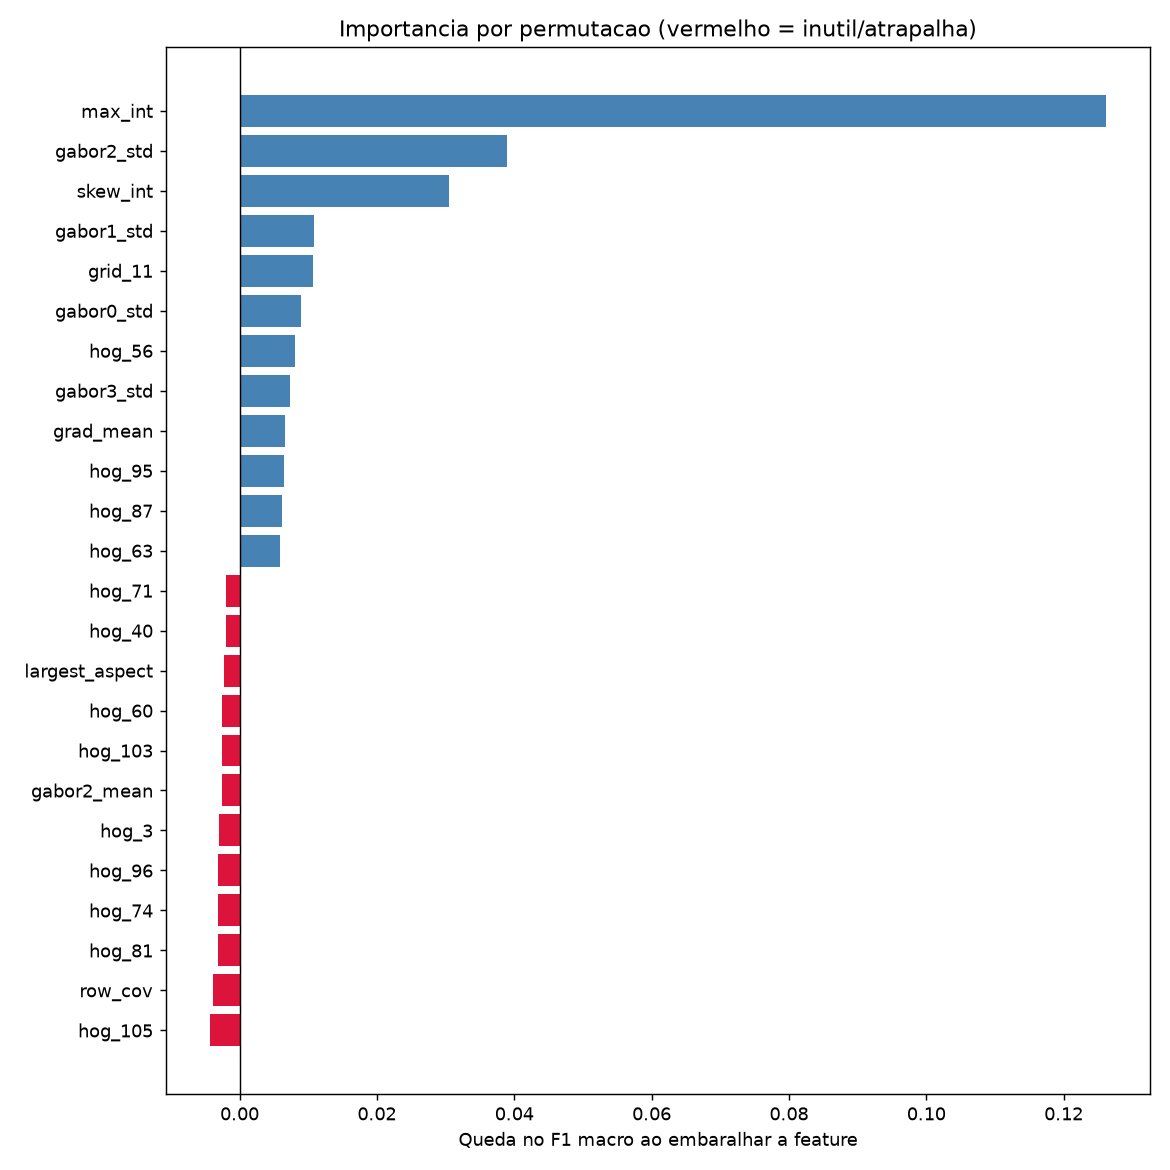
\includegraphics[width=0.7\linewidth]{importancia_features.png}
	\caption{Importância por permutação das características (vermelho = inútil ou prejudicial).}
	\label{fig:importancia}
\end{figure}

Removendo as características com importância $\leq 0$ e re-treinando o XGBoost, obtém-se um modelo mais enxuto sem perda relevante de desempenho, como mostra a Tabela \ref{tab:remocao}.

\begin{table}[H]
	\centering
	\caption{Desempenho do XGBoost com o conjunto completo vs reduzido de características.}
	\label{tab:remocao}
	\vspace{0.2cm}
	\renewcommand{\arraystretch}{1.2}
	\begin{tabular}{l c c c c c}
		\hline
		\textbf{Conjunto} & \textbf{Nº feat.} & \textbf{Acurácia} & \textbf{$\Delta$} & \textbf{F1 macro} & \textbf{$\Delta$} \\
		\hline
		Completo & 181 & 74,2\% & --   & 53,9\% & --   \\ \hline
		Reduzido & 115 & 73,9\% & -0,3 & 53,4\% & -0,5 \\
		\hline
	\end{tabular}
\end{table}

Das 181 características, 66 apresentaram importância nula ou negativa e foram removidas, restando 115. O desempenho praticamente não muda (-0,3 de acurácia e -0,5 de \textit{F1-score} macro, dentro da margem de ruído), confirmando que cerca de um terço das características era dispensável. O modelo reduzido é mais leve e rápido, sem custo relevante de qualidade.

\clearpage

\section{Solução com \textit{deep learning}}
Para a tarefa de identificação e classificação de anomalias em imagens termográficas, este trabalho emprega redes neurais convolucionais, dada a sua eficácia na extração de características em problemas de visão computacional. Optou-se pela utilização da arquitetura ResNet34, ajustada aos dados específicos da pesquisa por meio de técnicas de aprendizado por transferência.

A primeira etapa do desenvolvimento consistiu no pré-processamento e balanceamento da base de dados. Visando evitar o enviesamento do modelo em direção à classe majoritária, a categoria correspondente aos painéis operando em condições normais (\textit{No-Anomaly}) foi subamostrada aleatoriamente, sendo reduzida do seu total original de 10.000 amostras para 1.800 imagens. Além disso, para agrupar comportamentos térmicos equivalentes e mitigar redundâncias, algumas classes anômalas foram consolidadas. Ocorrências múltiplas de um mesmo defeito, registradas nos rótulos \textit{Cell-Multi}, \textit{Diode-Multi} e \textit{Hot-Spot-Multi}, foram incorporadas respectivamente às suas categorias raízes: \textit{Cell}, \textit{Diode} e \textit{Hot-Spot}. A distribuição estrutural do conjunto de dados após o processamento encontra-se detalhada na Tabela \ref{tab:dataset_atualizado}.

\begin{table}[htpb]
	\centering
	\caption{Distribuição atualizada das classes.}
	\label{tab:dataset_atualizado}
	\vspace{0.2cm}
	\begin{tabular}{l c}
		\hline
		\textbf{Classe} & \textbf{Número de Imagens} \\
		\hline
		Cell            & 3.165                      \\
		No-Anomaly      & 1.800                      \\
		Diode           & 1.674                      \\
		Vegetation      & 1.639                      \\
		Shadowing       & 1.056                      \\
		Cracking        & 940                        \\
		Offline-Module  & 827                        \\
		Hot-Spot        & 495                        \\
		Soiling         & 204                        \\
		\hline
	\end{tabular}
\end{table}

Com os dados organizados, o treinamento do modelo foi estruturado visando o melhor refinamento dos pesos da rede. Para realizar essa etapa, aplicou-se um método exploratório de busca pela melhor taxa de aprendizado, que permite identificar empiricamente a faixa de valores ideal onde a otimização atua de maneira mais eficiente e estável. A Figura \ref{fig:lr_find} ilustra o comportamento da função de perda em resposta à variação da taxa de aprendizado durante este teste.

\begin{figure}[H]
	\centering
	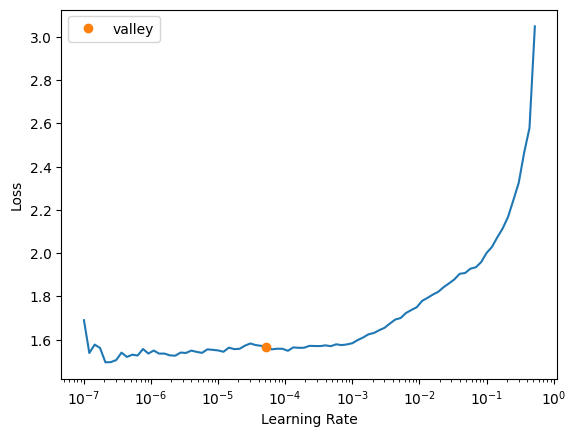
\includegraphics[width=0.5\linewidth]{lrfind.png}
	\caption{Função de perda em resposta à variação da taxa de aprendizado.}
	\label{fig:lr_find}
\end{figure}

A rede foi então treinada aplicando o ajuste fino com base na faixa ideal descoberta. Como resultado, o modelo ResNet34 alcançou uma precisão de 67\% e um \textit{F1-score} de 65\% no diagnóstico das classes. Os números não indicam onde o modelo acerta ou erra, portanto, para aprofundar a análise a respeito do desempenho de identificação por categoria, extraiu-se a matriz de confusão das predições em relação ao conjunto de teste, na qual é possível constatar a distribuição dos acertos, que estão concentrados na diagonal principal, e dos falsos positivos, conforme exposto na Figura \ref{fig:matriz_confusao}.

\begin{figure}[H]
	\centering
	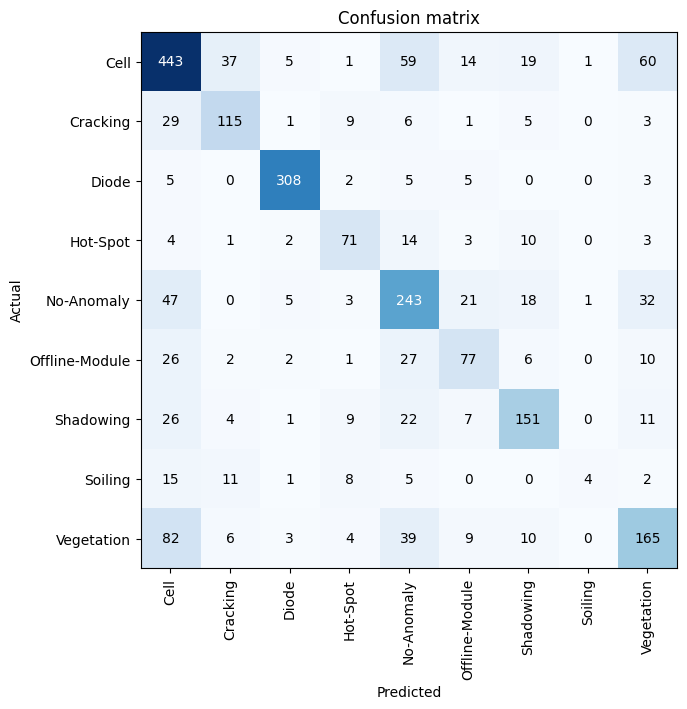
\includegraphics[width=0.8\linewidth]{matriz_confusao_dl.png}
	\caption{Matriz de confusão resultante das predições do modelo ResNet34.}
	\label{fig:matriz_confusao}
\end{figure}

Analisando a matriz, observa-se que o modelo apresenta um desempenho consistente nas categorias com maior volume de amostras. Contudo, o principal ponto de vulnerabilidade do classificador manifesta-se na classe \textit{Soiling}, que exibe uma taxa de erro mais acentuada em comparação às demais. Esse comportamento está diretamente associado à escassez de dados dessa categoria, que possui apenas 204 registros na base consolidada, limitando a capacidade da rede neural de extrair e generalizar características visuais para essa anomalia.

Para ilustrar o funcionamento do modelo, a Figura \ref{fig:amostras_resultados} demonstra uma amostra das classificações, comparando a resposta predita pela rede neural com o rótulo original da imagem.

\begin{figure}[H]
	\centering
	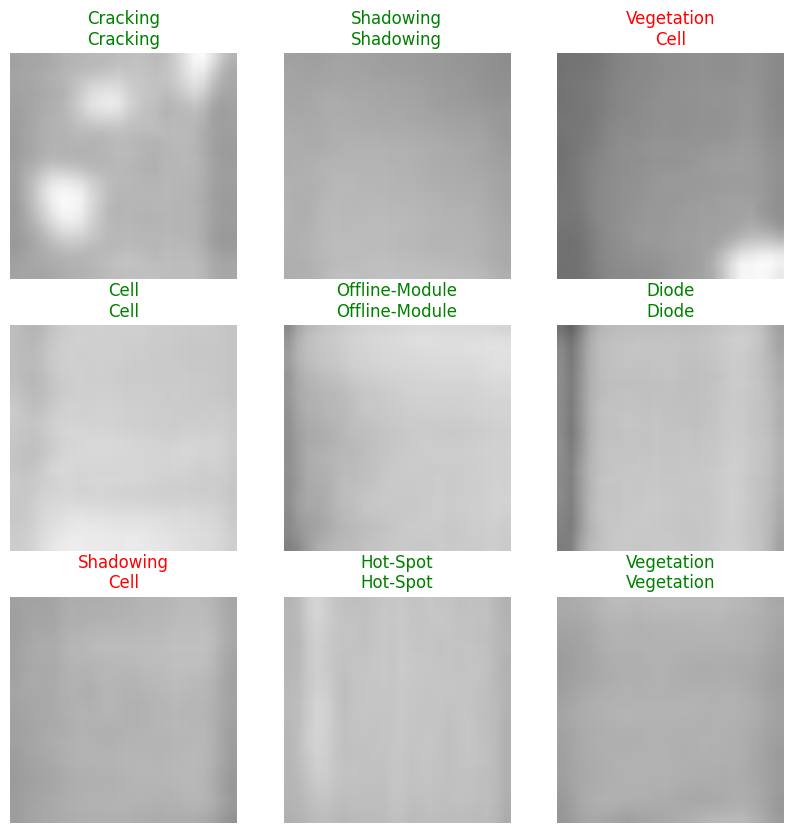
\includegraphics[width=0.8\linewidth]{resultados_predicao_dl.png}
	\caption{Amostra da operação do modelo.}
	\label{fig:amostras_resultados}
\end{figure}

Embora os resultados iniciais validem a viabilidade da técnica, limitações foram identificadas durante os experimentos. Tentativas preliminares de compensar o desbalanceamento do número de amostras por meio da aplicação de pesos resultaram em uma degradação no desempenho geral do modelo, reduzindo tanto a precisão quanto o \textit{F1-score}. Diante disso, como proposta de melhoria, sugere-se a exploração de técnicas de \textit{data augmentation}. Contudo, destaca-se que modificações artificiais de brilho e contraste devem ser evitadas, visto que em imagens termográficas, a intensidade dos pixels está relacionada à temperatura do módulo, de modo que alterações dessa natureza descaracterizariam os padrões reais das anomalias e da operação nominal dos painéis solares.
\clearpage

\section{Conclusão}

\end{document}
